% Created by tikzDevice version 0.11 on 2018-08-30 16:40:10
% !TEX encoding = UTF-8 Unicode
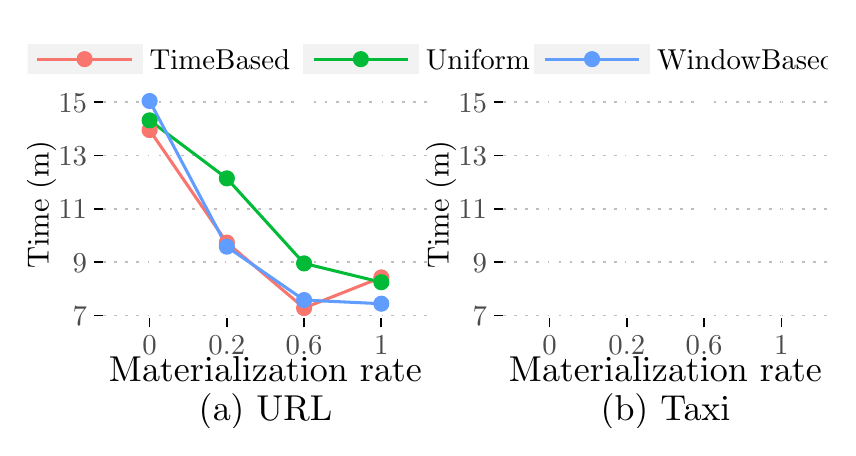
\begin{tikzpicture}[x=1pt,y=1pt]
\definecolor{fillColor}{RGB}{255,255,255}
\path[use as bounding box,fill=fillColor,fill opacity=0.00] (0,0) rectangle (289.08,144.54);
\begin{scope}
\path[clip] (  0.00,  0.00) rectangle (289.08,144.54);
\definecolor{fillColor}{RGB}{255,255,255}

\path[fill=fillColor] (-10.79,121.78) rectangle (299.87,144.54);
\end{scope}
\begin{scope}
\path[clip] (  0.00,  0.00) rectangle (289.08,144.54);
\definecolor{drawColor}{RGB}{255,255,255}
\definecolor{fillColor}{gray}{0.95}

\path[draw=drawColor,line width= 0.6pt,line join=round,line cap=round,fill=fillColor] ( -0.76,127.47) rectangle ( 41.92,138.85);
\end{scope}
\begin{scope}
\path[clip] (  0.00,  0.00) rectangle (289.08,144.54);
\definecolor{drawColor}{RGB}{248,118,109}

\path[draw=drawColor,line width= 1.1pt,line join=round] (  3.50,133.16) -- ( 37.65,133.16);
\end{scope}
\begin{scope}
\path[clip] (  0.00,  0.00) rectangle (289.08,144.54);
\definecolor{drawColor}{RGB}{248,118,109}
\definecolor{fillColor}{RGB}{248,118,109}

\path[draw=drawColor,line width= 0.4pt,line join=round,line cap=round,fill=fillColor] ( 20.58,133.16) circle (  2.71);
\end{scope}
\begin{scope}
\path[clip] (  0.00,  0.00) rectangle (289.08,144.54);
\definecolor{drawColor}{RGB}{255,255,255}
\definecolor{fillColor}{gray}{0.95}

\path[draw=drawColor,line width= 0.6pt,line join=round,line cap=round,fill=fillColor] ( 99.05,127.47) rectangle (141.73,138.85);
\end{scope}
\begin{scope}
\path[clip] (  0.00,  0.00) rectangle (289.08,144.54);
\definecolor{drawColor}{RGB}{0,186,56}

\path[draw=drawColor,line width= 1.1pt,line join=round] (103.32,133.16) -- (137.46,133.16);
\end{scope}
\begin{scope}
\path[clip] (  0.00,  0.00) rectangle (289.08,144.54);
\definecolor{drawColor}{RGB}{0,186,56}
\definecolor{fillColor}{RGB}{0,186,56}

\path[draw=drawColor,line width= 0.4pt,line join=round,line cap=round,fill=fillColor] (120.39,133.16) circle (  2.71);
\end{scope}
\begin{scope}
\path[clip] (  0.00,  0.00) rectangle (289.08,144.54);
\definecolor{drawColor}{RGB}{255,255,255}
\definecolor{fillColor}{gray}{0.95}

\path[draw=drawColor,line width= 0.6pt,line join=round,line cap=round,fill=fillColor] (182.61,127.47) rectangle (225.28,138.85);
\end{scope}
\begin{scope}
\path[clip] (  0.00,  0.00) rectangle (289.08,144.54);
\definecolor{drawColor}{RGB}{97,156,255}

\path[draw=drawColor,line width= 1.1pt,line join=round] (186.87,133.16) -- (221.02,133.16);
\end{scope}
\begin{scope}
\path[clip] (  0.00,  0.00) rectangle (289.08,144.54);
\definecolor{drawColor}{RGB}{97,156,255}
\definecolor{fillColor}{RGB}{97,156,255}

\path[draw=drawColor,line width= 0.4pt,line join=round,line cap=round,fill=fillColor] (203.94,133.16) circle (  2.71);
\end{scope}
\begin{scope}
\path[clip] (  0.00,  0.00) rectangle (289.08,144.54);
\definecolor{drawColor}{RGB}{0,0,0}

\node[text=drawColor,anchor=base west,inner sep=0pt, outer sep=0pt, scale=  1.04] at ( 44.08,129.58) {TimeBased};
\end{scope}
\begin{scope}
\path[clip] (  0.00,  0.00) rectangle (289.08,144.54);
\definecolor{drawColor}{RGB}{0,0,0}

\node[text=drawColor,anchor=base west,inner sep=0pt, outer sep=0pt, scale=  1.04] at (143.90,129.58) {Uniform};
\end{scope}
\begin{scope}
\path[clip] (  0.00,  0.00) rectangle (289.08,144.54);
\definecolor{drawColor}{RGB}{0,0,0}

\node[text=drawColor,anchor=base west,inner sep=0pt, outer sep=0pt, scale=  1.04] at (227.45,129.58) {WindowBased};
\end{scope}
\begin{scope}
\path[clip] (  0.00,  0.00) rectangle (144.54,121.78);
\definecolor{drawColor}{RGB}{255,255,255}
\definecolor{fillColor}{RGB}{255,255,255}

\path[draw=drawColor,line width= 0.6pt,line join=round,line cap=round,fill=fillColor] (  0.00,  0.00) rectangle (144.54,121.78);
\end{scope}
\begin{scope}
\path[clip] ( 27.32, 39.50) rectangle (144.54,121.78);
\definecolor{fillColor}{RGB}{255,255,255}

\path[fill=fillColor] ( 27.32, 39.50) rectangle (144.54,121.78);
\definecolor{drawColor}{RGB}{255,255,255}

\path[draw=drawColor,line width= 0.3pt,line join=round] ( 27.32, 50.15) --
	(144.54, 50.15);

\path[draw=drawColor,line width= 0.3pt,line join=round] ( 27.32, 69.43) --
	(144.54, 69.43);

\path[draw=drawColor,line width= 0.3pt,line join=round] ( 27.32, 88.71) --
	(144.54, 88.71);

\path[draw=drawColor,line width= 0.3pt,line join=round] ( 27.32,107.99) --
	(144.54,107.99);
\definecolor{drawColor}{RGB}{190,190,190}

\path[draw=drawColor,line width= 0.6pt,dash pattern=on 1pt off 3pt ,line join=round] ( 27.32, 40.51) --
	(144.54, 40.51);

\path[draw=drawColor,line width= 0.6pt,dash pattern=on 1pt off 3pt ,line join=round] ( 27.32, 59.79) --
	(144.54, 59.79);

\path[draw=drawColor,line width= 0.6pt,dash pattern=on 1pt off 3pt ,line join=round] ( 27.32, 79.07) --
	(144.54, 79.07);

\path[draw=drawColor,line width= 0.6pt,dash pattern=on 1pt off 3pt ,line join=round] ( 27.32, 98.35) --
	(144.54, 98.35);

\path[draw=drawColor,line width= 0.6pt,dash pattern=on 1pt off 3pt ,line join=round] ( 27.32,117.63) --
	(144.54,117.63);
\definecolor{drawColor}{RGB}{255,255,255}

\path[draw=drawColor,line width= 0.6pt,line join=round] ( 44.06, 39.50) --
	( 44.06,121.78);

\path[draw=drawColor,line width= 0.6pt,line join=round] ( 71.97, 39.50) --
	( 71.97,121.78);

\path[draw=drawColor,line width= 0.6pt,line join=round] ( 99.88, 39.50) --
	( 99.88,121.78);

\path[draw=drawColor,line width= 0.6pt,line join=round] (127.79, 39.50) --
	(127.79,121.78);
\definecolor{drawColor}{RGB}{248,118,109}

\path[draw=drawColor,line width= 1.1pt,line join=round] ( 44.06,107.53) --
	( 71.97, 66.88) --
	( 99.88, 43.24) --
	(127.79, 54.29);
\definecolor{drawColor}{RGB}{0,186,56}

\path[draw=drawColor,line width= 1.1pt,line join=round] ( 44.06,111.05) --
	( 71.97, 90.08) --
	( 99.88, 59.35) --
	(127.79, 52.55);
\definecolor{drawColor}{RGB}{97,156,255}

\path[draw=drawColor,line width= 1.1pt,line join=round] ( 44.06,118.04) --
	( 71.97, 65.40) --
	( 99.88, 46.11) --
	(127.79, 44.79);
\definecolor{drawColor}{RGB}{248,118,109}
\definecolor{fillColor}{RGB}{248,118,109}

\path[draw=drawColor,line width= 0.4pt,line join=round,line cap=round,fill=fillColor] ( 44.06,107.53) circle (  2.71);

\path[draw=drawColor,line width= 0.4pt,line join=round,line cap=round,fill=fillColor] ( 71.97, 66.88) circle (  2.71);

\path[draw=drawColor,line width= 0.4pt,line join=round,line cap=round,fill=fillColor] ( 99.88, 43.24) circle (  2.71);

\path[draw=drawColor,line width= 0.4pt,line join=round,line cap=round,fill=fillColor] (127.79, 54.29) circle (  2.71);
\definecolor{drawColor}{RGB}{0,186,56}
\definecolor{fillColor}{RGB}{0,186,56}

\path[draw=drawColor,line width= 0.4pt,line join=round,line cap=round,fill=fillColor] ( 44.06,111.05) circle (  2.71);

\path[draw=drawColor,line width= 0.4pt,line join=round,line cap=round,fill=fillColor] ( 71.97, 90.08) circle (  2.71);

\path[draw=drawColor,line width= 0.4pt,line join=round,line cap=round,fill=fillColor] ( 99.88, 59.35) circle (  2.71);

\path[draw=drawColor,line width= 0.4pt,line join=round,line cap=round,fill=fillColor] (127.79, 52.55) circle (  2.71);
\definecolor{drawColor}{RGB}{97,156,255}
\definecolor{fillColor}{RGB}{97,156,255}

\path[draw=drawColor,line width= 0.4pt,line join=round,line cap=round,fill=fillColor] ( 44.06,118.04) circle (  2.71);

\path[draw=drawColor,line width= 0.4pt,line join=round,line cap=round,fill=fillColor] ( 71.97, 65.40) circle (  2.71);

\path[draw=drawColor,line width= 0.4pt,line join=round,line cap=round,fill=fillColor] ( 99.88, 46.11) circle (  2.71);

\path[draw=drawColor,line width= 0.4pt,line join=round,line cap=round,fill=fillColor] (127.79, 44.79) circle (  2.71);
\end{scope}
\begin{scope}
\path[clip] (  0.00,  0.00) rectangle (289.08,144.54);
\definecolor{drawColor}{gray}{0.30}

\node[text=drawColor,anchor=base east,inner sep=0pt, outer sep=0pt, scale=  1.04] at ( 21.47, 36.93) {7};

\node[text=drawColor,anchor=base east,inner sep=0pt, outer sep=0pt, scale=  1.04] at ( 21.47, 56.21) {9};

\node[text=drawColor,anchor=base east,inner sep=0pt, outer sep=0pt, scale=  1.04] at ( 21.47, 75.49) {11};

\node[text=drawColor,anchor=base east,inner sep=0pt, outer sep=0pt, scale=  1.04] at ( 21.47, 94.77) {13};

\node[text=drawColor,anchor=base east,inner sep=0pt, outer sep=0pt, scale=  1.04] at ( 21.47,114.05) {15};
\end{scope}
\begin{scope}
\path[clip] (  0.00,  0.00) rectangle (289.08,144.54);
\definecolor{drawColor}{RGB}{0,0,0}

\path[draw=drawColor,line width= 0.6pt,line join=round] ( 24.07, 40.51) --
	( 27.32, 40.51);

\path[draw=drawColor,line width= 0.6pt,line join=round] ( 24.07, 59.79) --
	( 27.32, 59.79);

\path[draw=drawColor,line width= 0.6pt,line join=round] ( 24.07, 79.07) --
	( 27.32, 79.07);

\path[draw=drawColor,line width= 0.6pt,line join=round] ( 24.07, 98.35) --
	( 27.32, 98.35);

\path[draw=drawColor,line width= 0.6pt,line join=round] ( 24.07,117.63) --
	( 27.32,117.63);
\end{scope}
\begin{scope}
\path[clip] (  0.00,  0.00) rectangle (289.08,144.54);
\definecolor{drawColor}{RGB}{0,0,0}

\path[draw=drawColor,line width= 0.6pt,line join=round] ( 44.06, 36.25) --
	( 44.06, 39.50);

\path[draw=drawColor,line width= 0.6pt,line join=round] ( 71.97, 36.25) --
	( 71.97, 39.50);

\path[draw=drawColor,line width= 0.6pt,line join=round] ( 99.88, 36.25) --
	( 99.88, 39.50);

\path[draw=drawColor,line width= 0.6pt,line join=round] (127.79, 36.25) --
	(127.79, 39.50);
\end{scope}
\begin{scope}
\path[clip] (  0.00,  0.00) rectangle (289.08,144.54);
\definecolor{drawColor}{gray}{0.30}

\node[text=drawColor,anchor=base,inner sep=0pt, outer sep=0pt, scale=  1.04] at ( 44.06, 26.49) {0};

\node[text=drawColor,anchor=base,inner sep=0pt, outer sep=0pt, scale=  1.04] at ( 71.97, 26.49) {0.2};

\node[text=drawColor,anchor=base,inner sep=0pt, outer sep=0pt, scale=  1.04] at ( 99.88, 26.49) {0.6};

\node[text=drawColor,anchor=base,inner sep=0pt, outer sep=0pt, scale=  1.04] at (127.79, 26.49) {1};
\end{scope}
\begin{scope}
\path[clip] (  0.00,  0.00) rectangle (289.08,144.54);
\definecolor{drawColor}{RGB}{0,0,0}

\node[text=drawColor,anchor=base,inner sep=0pt, outer sep=0pt, scale=  1.30] at ( 85.93, 16.53) {Materialization rate};

\node[text=drawColor,anchor=base,inner sep=0pt, outer sep=0pt, scale=  1.30] at ( 85.93,  2.49) { (a) URL};
\end{scope}
\begin{scope}
\path[clip] (  0.00,  0.00) rectangle (289.08,144.54);
\definecolor{drawColor}{RGB}{0,0,0}

\node[text=drawColor,rotate= 90.00,anchor=base,inner sep=0pt, outer sep=0pt, scale=  1.10] at (  7.58, 80.64) {Time (m)};
\end{scope}
\begin{scope}
\path[clip] (144.54,  0.00) rectangle (289.08,121.78);
\definecolor{drawColor}{RGB}{255,255,255}
\definecolor{fillColor}{RGB}{255,255,255}

\path[draw=drawColor,line width= 0.6pt,line join=round,line cap=round,fill=fillColor] (144.54,  0.00) rectangle (289.08,121.78);
\end{scope}
\begin{scope}
\path[clip] (171.86, 39.50) rectangle (289.08,121.78);
\definecolor{fillColor}{RGB}{255,255,255}

\path[fill=fillColor] (171.86, 39.50) rectangle (289.08,121.78);
\definecolor{drawColor}{RGB}{255,255,255}

\path[draw=drawColor,line width= 0.3pt,line join=round] (171.86, 50.15) --
	(289.08, 50.15);

\path[draw=drawColor,line width= 0.3pt,line join=round] (171.86, 69.43) --
	(289.08, 69.43);

\path[draw=drawColor,line width= 0.3pt,line join=round] (171.86, 88.71) --
	(289.08, 88.71);

\path[draw=drawColor,line width= 0.3pt,line join=round] (171.86,107.99) --
	(289.08,107.99);
\definecolor{drawColor}{RGB}{190,190,190}

\path[draw=drawColor,line width= 0.6pt,dash pattern=on 1pt off 3pt ,line join=round] (171.86, 40.51) --
	(289.08, 40.51);

\path[draw=drawColor,line width= 0.6pt,dash pattern=on 1pt off 3pt ,line join=round] (171.86, 59.79) --
	(289.08, 59.79);

\path[draw=drawColor,line width= 0.6pt,dash pattern=on 1pt off 3pt ,line join=round] (171.86, 79.07) --
	(289.08, 79.07);

\path[draw=drawColor,line width= 0.6pt,dash pattern=on 1pt off 3pt ,line join=round] (171.86, 98.35) --
	(289.08, 98.35);

\path[draw=drawColor,line width= 0.6pt,dash pattern=on 1pt off 3pt ,line join=round] (171.86,117.63) --
	(289.08,117.63);
\definecolor{drawColor}{RGB}{255,255,255}

\path[draw=drawColor,line width= 0.6pt,line join=round] (188.60, 39.50) --
	(188.60,121.78);

\path[draw=drawColor,line width= 0.6pt,line join=round] (216.51, 39.50) --
	(216.51,121.78);

\path[draw=drawColor,line width= 0.6pt,line join=round] (244.42, 39.50) --
	(244.42,121.78);

\path[draw=drawColor,line width= 0.6pt,line join=round] (272.33, 39.50) --
	(272.33,121.78);

\path[] (188.60,107.53) --
	(216.51, 66.88) --
	(244.42, 43.24) --
	(272.33, 54.29);

\path[] (188.60,111.05) --
	(216.51, 90.08) --
	(244.42, 59.35) --
	(272.33, 52.55);

\path[] (188.60,118.04) --
	(216.51, 65.40) --
	(244.42, 46.11) --
	(272.33, 44.79);
\end{scope}
\begin{scope}
\path[clip] (  0.00,  0.00) rectangle (289.08,144.54);
\definecolor{drawColor}{gray}{0.30}

\node[text=drawColor,anchor=base east,inner sep=0pt, outer sep=0pt, scale=  1.04] at (166.01, 36.93) {7};

\node[text=drawColor,anchor=base east,inner sep=0pt, outer sep=0pt, scale=  1.04] at (166.01, 56.21) {9};

\node[text=drawColor,anchor=base east,inner sep=0pt, outer sep=0pt, scale=  1.04] at (166.01, 75.49) {11};

\node[text=drawColor,anchor=base east,inner sep=0pt, outer sep=0pt, scale=  1.04] at (166.01, 94.77) {13};

\node[text=drawColor,anchor=base east,inner sep=0pt, outer sep=0pt, scale=  1.04] at (166.01,114.05) {15};
\end{scope}
\begin{scope}
\path[clip] (  0.00,  0.00) rectangle (289.08,144.54);
\definecolor{drawColor}{RGB}{0,0,0}

\path[draw=drawColor,line width= 0.6pt,line join=round] (168.61, 40.51) --
	(171.86, 40.51);

\path[draw=drawColor,line width= 0.6pt,line join=round] (168.61, 59.79) --
	(171.86, 59.79);

\path[draw=drawColor,line width= 0.6pt,line join=round] (168.61, 79.07) --
	(171.86, 79.07);

\path[draw=drawColor,line width= 0.6pt,line join=round] (168.61, 98.35) --
	(171.86, 98.35);

\path[draw=drawColor,line width= 0.6pt,line join=round] (168.61,117.63) --
	(171.86,117.63);
\end{scope}
\begin{scope}
\path[clip] (  0.00,  0.00) rectangle (289.08,144.54);
\definecolor{drawColor}{RGB}{0,0,0}

\path[draw=drawColor,line width= 0.6pt,line join=round] (188.60, 36.25) --
	(188.60, 39.50);

\path[draw=drawColor,line width= 0.6pt,line join=round] (216.51, 36.25) --
	(216.51, 39.50);

\path[draw=drawColor,line width= 0.6pt,line join=round] (244.42, 36.25) --
	(244.42, 39.50);

\path[draw=drawColor,line width= 0.6pt,line join=round] (272.33, 36.25) --
	(272.33, 39.50);
\end{scope}
\begin{scope}
\path[clip] (  0.00,  0.00) rectangle (289.08,144.54);
\definecolor{drawColor}{gray}{0.30}

\node[text=drawColor,anchor=base,inner sep=0pt, outer sep=0pt, scale=  1.04] at (188.60, 26.49) {0};

\node[text=drawColor,anchor=base,inner sep=0pt, outer sep=0pt, scale=  1.04] at (216.51, 26.49) {0.2};

\node[text=drawColor,anchor=base,inner sep=0pt, outer sep=0pt, scale=  1.04] at (244.42, 26.49) {0.6};

\node[text=drawColor,anchor=base,inner sep=0pt, outer sep=0pt, scale=  1.04] at (272.33, 26.49) {1};
\end{scope}
\begin{scope}
\path[clip] (  0.00,  0.00) rectangle (289.08,144.54);
\definecolor{drawColor}{RGB}{0,0,0}

\node[text=drawColor,anchor=base,inner sep=0pt, outer sep=0pt, scale=  1.30] at (230.47, 16.53) {Materialization rate};

\node[text=drawColor,anchor=base,inner sep=0pt, outer sep=0pt, scale=  1.30] at (230.47,  2.49) { (b) Taxi};
\end{scope}
\begin{scope}
\path[clip] (  0.00,  0.00) rectangle (289.08,144.54);
\definecolor{drawColor}{RGB}{0,0,0}

\node[text=drawColor,rotate= 90.00,anchor=base,inner sep=0pt, outer sep=0pt, scale=  1.10] at (152.12, 80.64) {Time (m)};
\end{scope}
\end{tikzpicture}
